\documentclass[a4paper]{article}
\usepackage[paperwidth=180mm,paperheight=285mm,left=3cm,top=4cm,right=3cm,bottom=2cm,head=2.0cm,includefoot]{geometry}
\usepackage{makeidx}
\usepackage[spanish]{babel}
\usepackage[utf8]{inputenc}
\usepackage{amsmath}
\usepackage{url}
\usepackage{fancyvrb}
\usepackage{babelbib}
\usepackage{graphicx}
\usepackage{lscape}
\usepackage{fancyhdr}
\graphicspath{ {img/} }

\newtheorem{definicion}{Definición} 

\urldef{\mails}\path|{fbarrios,fjlopez}@fi.uba.ar| 

\title{Módulo de resúmenes automáticos basado en TextRank con integración a Gensim}
\author{Barrios, Federico \and López, Federico}

\lhead{
\includegraphics[scale=0.06]{./logo_fiuba.pdf}}
\chead{Módulo de resúmenes automáticos basado\linebreak en TextRank con integración a Gensim}
\rhead{}

\lfoot{Barrios - López}
\rfoot{\thepage}
\cfoot{Mayo, 2015}

\begin{document}

\thispagestyle{empty}
% T\'itulo del documento.
\begin{center}
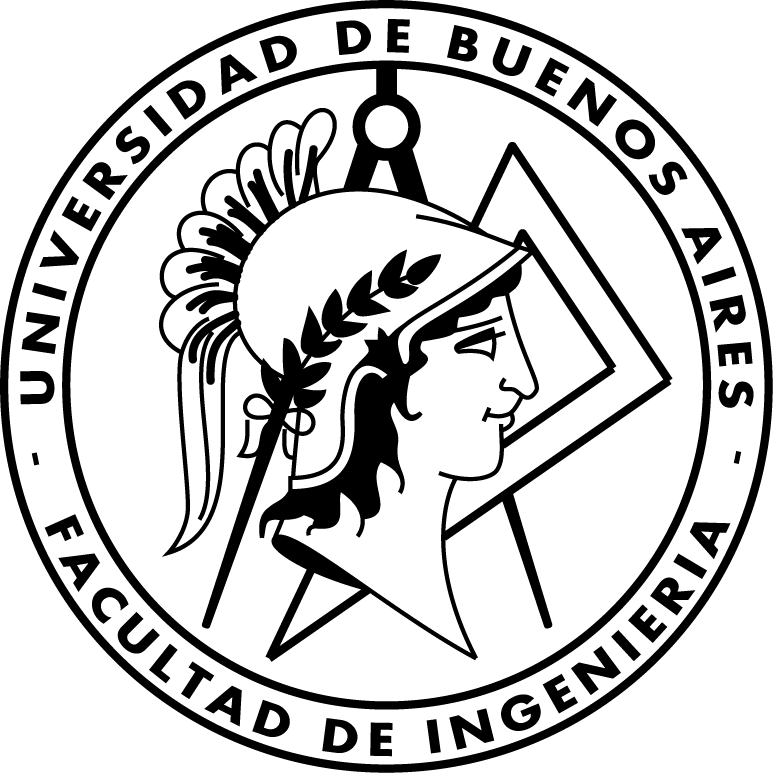
\includegraphics{./logo-fiuba.png}\\
\vspace{1cm}
\textsc{\LARGE Universidad de Buenos Aires}\\[0.3cm]
\textsc{\LARGE Facultad de Ingenier\'ia}\\[1.2cm]
\textsc{\LARGE Módulo de resúmenes automáticos basado en TextRank con integración a Gensim}\\[0.3cm]
\end{center}

\vspace{20 mm}

\begin{flushright}
{\large
Barrios, Federico -- 92954\\
L\'opez, Federico -- 92278\\[0.1cm]
\vspace{2cm}
Mayo, 2015}
\end{flushright}

\pagestyle{fancy}
\newpage

\footnotesize


\newpage
\setcounter{page}{1}
\tableofcontents

\newpage
\section{Motivación}
Los resúmenes automatizados son muy utilizados en tareas relacionadas con el procesamiento de lenguaje natural y de aprendizaje automático. Su uso en motores de búsqueda, por ejemplo, mejora la eficiencia de indexación de textos y a su vez asiste en la presentación de resultados de manera efectiva. El incremento en la cantidad de información disponible en Internet ha intensificado su utilización en los últimos años y, en consecuencia, se ha dedicado enorme esfuerzo para mejorar los algoritmos existentes. 


\section{Objetivos}
El presente trabajo consta de tres objetivos principales:
\begin{itemize}
\item Desarrollar el módulo para generar resúmenes automáticos usando un algoritmo conocido.
\item Analizar, diseñar e implementar modificaciones para intentar mejorar el rendimiento del algoritmo seleccionado.
\item Integrar las implementaciones a una herramienta de código abierto de procesamiento del lenguaje natural.
\end{itemize}

\section{Introducción teórica}

\subsection{Resúmenes: generación y clasificación}
Un resumen es una reducción a términos breves y precisos de lo esencial de una fuente de información. Su objetivo es el de extraer contenido intentando sintetizar sus conceptos más importantes, y su uso es altamente benéfico en tareas de aprendizaje debido a que:
\begin{itemize}
\item Facilitan la selección de información,
\item Acortan tiempos de lectura,
\item Simplifican búsquedas en textos,
\item Optimizan la creación de índices.
\end{itemize}

La investigación indica, además, que contribuyen en tareas automatizadas: su utilización para presentar resultados de motores de búsquedas atrajo el interés de académicos desde principios de la década del 2000, convirtiéndose hoy en día en una funcionalidad básica de los principales buscadores de Internet.

Sin embargo, si bien esta tarea puede no resultar costosa para un ser humano, durante muchos años fue considerada como difícil de automatizar. Este tema es uno de los que investiga el campo de procesamiento de lenguaje natural, dedicado a facilitar la interacción entre las computadoras y los seres humanos.


\subsubsection{Enfoque abstractivo y extractivo}

Existen dos métodos para generar resúmenes automatizados: abstractivos y extractivos.

Los primeros se construyen regenerando el contenido extraído del texto original; esto es, se reformulan las frases por medio de técnicas de generación de lenguaje natural: fusión, combinación o supresión de términos. De esta manera, se obtienen pasajes que en principio no pertenecían al texto de origen, similar al modo en que lo harían las personas. 

Por el contrario, los resúmenes extractivos se crean a partir de la selección de un conjunto de palabras u oraciones consideradas sobresalientes en el texto original. Las oraciones se obtienen literalmente, se unen libremente, y se presentan con el objetivo de crear un resumen del texto.

Las técnicas abstractivas son un área de creciente interés. Sin embargo, debido a la complejidad y las restricciones técnicas aparejadas, la investigación se ha volcado hacia el enfoque extractivo.


\subsubsection{Aprendizaje supervisado y no supervisado}
En el campo del aprendizaje automático, a los algoritmos que requieren de un conjunto de entrenamiento con datos etiquetados se denominan supervisados. Analizando estos ejemplos de entrenamiento, el sistema infiere funciones que pueden ser usadas para aplicarlas a nueva información.

Por el contrario, a los algoritmos que no son entrenados se los denomina no supervisados. Este grupo utiliza técnicas para encontrar patrones o grupos ocultos en los datos a analizar.


\subsubsection{Fuente de los datos}
Los algoritmos de generación de resúmenes también se categorizan de acuerdo a la cantidad de documentos que se toman como fuente, determinando sumarización de un documento y multi-documento.

Para este último caso se proporcionan textos con una temática afín. El resumen resultante permite a los lectores familiarizarse rápidamente con los tópicos principales de una colección de documentos.


\subsubsection{Propósito del resumen}
Los resúmenes de documentos pueden crearse de manera genérica o bien basados en consultas. 

Aquéllos resúmenes basados en consultas favorecen temas o aspectos específicos de un texto, de acuerdo a dicha consulta; teniendo en cuenta sus palabras clave o los tópicos a los que hace referencia. Los resúmenes genéricos, por otro lado, proporcionan los temas más relevantes tratados en el texto por sí solo.


\subsection{Extracción de palabras claves}
La extracción de palabras claves consiste en identificar el conjunto de términos que mejor describen a un documento de manera automatizada. Esto sirve como introducción a sus conceptos más relevantes, pues uno de los primeros pasos para modelar el conocimiento de una comunidad es tomar vocabulario del dominio. Es por ello que se han estudiado métodos para extraer este léxico técnico en base a documentos del área o comunidad en estudio.

Dichas palabras se pueden utilizar para construir índices de colecciones, clasificar textos, extraer terminología de dominio específica, o incluso pueden servir como un breve resumen.

El enfoque más sencillo para esta tarea ha empleado un criterio basado en la frecuencia de las palabras. Sin embargo, se han investigado otras debido a los malos resultados de esta técnica. Las principales se basan en métodos supervisados, donde el sistema es entrenado para reconocer palabras claves tomando en cuenta cuestiones sintácticas y/o léxicas. 

En la sección ‘TextRank para palabras claves’ se analiza y desarrolla la aplicación de TextRank como método no supervisado para esta tarea. Los resultados obtenidos se equiparan los de las técnicas principales en el área.


\section{Trabajo previo}
Se ha visto un gran avance en el campo de la generación automática de resúmenes desde finales de 1960 hasta la actualidad \cite{miranda}. Los métodos tradicionales tienen en cuenta la frecuencia de palabras o frases introductorias para identificar las oraciones más sobresalientes del texto. También, se han desarrollado modelos estadísticos basados en corpus de entrenamiento para combinar varias heurísticas: palabras clave, posición de las oraciones, longitud de las oraciones, frecuencia de palabras y palabras contenidas en los títulos \cite{hovy}. Otros enfoques se basan en la representación del texto en forma de grafo. Las oraciones importantes y los conceptos son las entidades altamente conectadas y, por esto, forman parte del resumen \cite{barzilay}. De igual modo, se ha propuesto analizar la estructura discursiva y extraer las relaciones retóricas entre las diferentes unidades textuales, y así separar las principales de las secundarias para descubrir las unidades que juegan un papel preponderante dentro de la estructura discursiva \cite{marcu}.

En la línea de representación del texto como un grafo conectado, se usan técnicas de Recuperación de Información para identificar oraciones similares y determinar las más importantes, que formarán al resumen final \cite{salton}. El enfoque propuesto, tanto por Mihalcea \& Tarau como por Erkan \& Radev \cite{erkan}, consiste en utilizar el prestigio de las unidades léxicas (oraciones o palabras) dentro del grafo. Dicha técnica ha sido la adoptada en el presente trabajo.


\section{Herramientas y fundamentos}

\subsection{PageRank}
PageRank es un algoritmo creado por Larry Page y Sergey Brin, fundadores de Google, en 1996, como parte de una investigación sobre motores de búsqueda. Su objetivo es asignar un valor numérico a cada nodo en una red, con el propósito de medir la importancia relativa de cada elemento del conjunto. Para esto analiza los vínculos que componen la red. La idea subyacente es que los nodos más relevantes de la red serán los que tengan la mayor cantidad y calidad de conexiones con otros nodos. 

En sus orígenes, PageRank fue pensado para aplicarse sobre la red de Internet (World Wide Web), pero puede aplicarse a cualquier otra red para estimar sus elementos principales. En términos matemáticos, PageRank brinda una manera iterativa de calcular el autovector principal de la matriz de adyacencia del grafo. Esto da como resultado la distribución de probabilidad de acceder a los nodos de la red, navegando de manera aleatoria a través de los vínculos o aristas.

Una de las características más notables del algoritmo es que toma en cuenta la información global de toda la red, y no sólo lo concerniente a cada nodo en particular. Si se arma un grafo en base a un documento, con las unidades léxicas o semánticas como vértices, se puede aplicar PageRank para priorizar los nodos principales. De esta manera, se pueden obtener las oraciones o palabras principales, utilizando información proveniente de todo el texto. En este enfoque está basado TextRank.


\subsection{TextRank}
TextRank es un algoritmo no supervisado basado en grafos para realizar resúmenes automáticos extractivos y/u obtener palabras claves de un texto. Fue presentado en 2004 por Rada Mihalcea y Paul Tarau en el paper “TextRank: Bringing Order into Texts” \cite{mihalcea-tarau}.

El algoritmo aplica una variación de PageRank \cite{pageetal98} sobre un grafo especialmente diseñado para la tarea. De esta manera permite explotar la estructura del texto, identificando los conceptos principales, sin necesidad de datos previos de entrenamiento. Debido a que se basa en PageRank, se sirve de la noción del “prestigio” o “recomendación” entre los elementos del grafo. Por este motivo, TextRank puede ser aplicado a cualquier texto, incluso en distintos idiomas, generando un resumen basado sólo en las propiedades intrínsecas del texto.

El algoritmo modela el texto en base a un grafo, y luego, busca crear relaciones significativas (aristas) entre las entidades léxicas (vértices). Dependiendo de la aplicación que se desee dar al algoritmo, las entidades pueden ser palabras, frases, oraciones, párrafos, entre otros. De manera similar, también debe definirse el tipo de relación que se usa para unir los vértices: semántica, contextual, de superposición, y demás.

Los pasos principales que se llevan a cabo son los siguientes:

\begin{enumerate}
\item Identificar las unidades del texto (palabras u oraciones) y agregarlas al grafo como vértices.
\item Identificar relaciones que conectan a estas unidades, y agregarlas al grafo como aristas entre los vértices. Las aristas pueden ser dirigidas o no, y ponderadas o no.
\item Aplicar PageRank para asignarle un puntaje a cada vértice.
\item Ordenar los vértices de acuerdo al puntaje y utilizarlo para armar el resumen de acuerdo a algún criterio.
\end{enumerate}

Las particularidades de los casos de creación de resúmenes y extracción de palabras claves se analizan en la sección 'Implementación'.


\subsection{Gensim}
Es una biblioteca de código libre, escrita en Python para el modelaje de tópicos y la indexación de documentos que está diseñada para trabajar con conjuntos de textos de gran tamaño. Su uso se ha expandido tanto en lo comercial como lo académico, apuntando especialmente al área de procesamiento del lenguaje natural y a la búsqueda y recuperación de la información.

Gensim utiliza un paradigma muy poderoso en el área de procesamiento de lenguaje natural, denominado VSM (modelo de espacio de vectores), en el cual se representan los documentos de un corpus como vectores de un espacio de muchas dimensiones. Esta representación explota la idea de que los textos en el área del modelado de tópicos se pueden expresar según un número de conceptos, lo que aumenta la eficiencia y también ayuda a eliminar ruido.

La biblioteca está diseñada para proveer independencia del tamaño del corpus, es decir, para poder analizar textos que sean más grandes que la memoria RAM del sistema. El proyecto, además apunta a exponer una interfaz mínima e intuitiva utilizando terminología de procesamiento de lenguaje.

Gensim proporciona implementaciones de algoritmos como TF-IDF, análisis semántico latente, proyecciones aleatorias y alocación de Dirichlet latente.


\subsection{Evaluación de resúmenes}
La herramienta por defecto para evaluar los sistemas generadores de resúmenes es Rouge (Recall-Oriented Understudy for Gisting Evaluation). Este método fue desarrollado en la universidad de Southern California para automatizar la comparación entre resúmenes generados por el sistema bajo evaluación contra otros (ideales) escritos por seres humanos, tomados como referencia.

Históricamente, los puntajes asignados en tareas de competencias como DUC fueron manuales; juzgando coherencia, capitalización, cohesión, consistencia y contenido \cite{duc2002}. Todo este trabajo es caro y difícil de coordinar, demandando de al menos 3.000 horas hombre. El surgimiento de Rouge atiende la necesidad de automatizar ese proceso, reemplazando un método llamado BLEU, cuyos resultados no siempre se correlacionaban con los asignados por los jurados.

El mecanismo de funcionamiento de los métodos del paquete Rouge consiste en calcular la sensibilidad (recall) de unidades léxicas entre los resúmenes de sistema y los de referencia. Se generan así diferentes métricas:
\begin{itemize}
\item Rouge-N: cuando se tienen en cuenta n-gramas (n palabras). Este método favorece a documentos con palabras compartidas por más candidatos.
\item Rouge-L: cuando se tiene en cuenta la subsecuencia máxima común (LCS, longest common subsequence). Este método propone que un conjunto de documentos va a ser más parecido mientras más larga sea la subsecuencia común máxima.
\item Rouge-W: le asigna pesos a las subsecuencias según su largo.
\item Rouge-S: es similar a Rouge-2, teniendo en cuenta bigramas pero permitiendo una cantidad arbitraria de espacios entre palabras.
\item Rouge-SU: extiende la idea de Rouge-S, pero además le otorga valor a las palabras que haya en común, sin importar que no verifiquen un orden.
\end{itemize}

Rouge asigna un puntaje entre cero y uno a un esquema de evaluación conformado por una serie de documentos generados y sus referencias. Por diseño, se espera que buenos resúmenes tengan puntajes más altos; pero inevitablemente se requiere de trabajo humano para proveer las referencias.

Para verificar el funcionamiento de Rouge se han usado las bases de datos de las conferencias DUC de los años 2001, 2002 y 2003. Se compararon las evaluaciones con los puntajes otorgados manualmente por los jurados para encontrar que todas las métricas arrojan muy buenos resultados; y a partir de la edición 2004 las evaluaciones se llevan a cabo usando exclusivamente Rouge.


\section{Implementación}
\subsection{Preprocesamiento}
El preprocesamiento del texto es una parte esencial en cualquier sistema que trate con datos del lenguaje natural. En esta fase se identifican las unidades léxicas que serán analizadas por la aplicación en las etapas subsiguientes. 

La calidad de este proceso tendrá un gran impacto en los resultados obtenidos. Es por ello que se deben seleccionar unidades léxicas significativas. Es decir, aquellas que contengan las características lingüísticas relevantes para el caso en estudio. A su vez, se deben filtrar las que no aportan información útil. En este proceso también, se unifica la codificación que pudiera existir en los distintos textos.

Aquí se detallan las etapas principales.

\subsubsection{Separación del texto}
Esta etapa, también conocida como tokenización consiste en separar el texto en oraciones o palabras. Separar palabras suele resultar más sencillo, dado que los espacios en blanco son una buena aproximación como límite de separación. Se debe tener un tratamiento especial de los casos tales como “can’t” o “don’t” en idiomas como el inglés.

Separar por oraciones suele ser caso más complejo. Definir los límites es una cuestión realmente problemática en el área del lenguaje natural. Generalmente se utilizan los símbolos .!? como separadores, pero se deben tratar con cuidado excepciones como \textit{Ph.D., Dr., Lic., \$19.99, p.m. o RR.HH}.

El enfoque más utilizado para resolver esta cuestión se basa en la aplicación de expresiones regulares teniendo en cuenta reglas como las siguientes:
\begin{enumerate}
\item El punto (“.”) finaliza una oración si la siguiente palabra comienza con mayúscula.
\item Si la palabra precedente al punto pertenece a un listado de abreviaturas preestablecido, entonces no termina la oración.
\end{enumerate}

Otras alternativas consisten en el uso de algoritmos entrenados con datos específicos del área sobre la cual se esté trabajando.


\subsubsection{Filtrado}
Las palabras más frecuentes muchas veces no tienen tanto significado por sí solas. Por ejemplo: “el, los, un, por, en”. En muchas tareas de procesamiento de lenguaje natural estas palabras aportan “ruido”, y por lo tanto se las debe quitar. 

La forma de filtrar palabras consiste en crear una lista de “palabras prohibidas” (\textit{stopwords} en inglés). Luego se recorre el texto, eliminando dichos términos.


\subsubsection{Stemming}
El proceso de \textit{stemming} (del inglés stem, significa raíz) o \textit{lemmatización} consiste en quitar la desinencia de las diferentes términos, para llevarlos a su raíz. Por ejemplo, las palabras “cantar, cantaba, cantando”, se las puede llevar todas a “canta”. Esta etapa se lleva a cabo con el objetivo de que el algoritmo detecte cuando se están tratando los mismos conceptos, dado que se utilizan las mismas palabras.

El stemming es un proceso complejo dado que puede haber muchos casos excepcionales, y se necesitan reglas muy diferentes para cada idioma. El stemmer más usado en inglés es el Porter Stemmer. Para cada idioma existe una adaptación. Sin embargo, todos estos algoritmos tienen cierta tasa de error.



\subsection{TextRank para extracción de oraciones}
El problema de la extracción de oraciones apunta a identificar las secuencias más representativas del texto. Para este caso, las unidades tomadas para aplicar el algoritmo serán oraciones completas \cite{introductionir}.

Inicialmente, se construye un grafo en base al texto. En este caso, se agrega cada oración como vértice. Para crear las aristas con su peso correspondiente, se debe definir una función de similitud entre dos oraciones dadas. Esta función de similitud será la que dicte cuánto una oración “recomienda” a otra, dado que ambas poseen contenidos similares y abordan los mismos conceptos.
    
La función utilizada formalmente se define de la siguiente manera:

\begin{definicion}
Sean $S_i$, $S_j$ dos oraciones representadas por un conjunto de $n$ palabras que en 
$S_i$ aparecen como $S_i = w_{1}^{i}, w_{2}^{i},..., w_{n}^{i}$, la función de similitud para $S_i$, $S_j$ se define como:

\begin{equation}
Similitud(S_{i},S_{j}) = \frac{ | \{   w_{k} | w_{k} \in S_{i} \& w_{k} \in S_{j}   \}  | }    
                              {  log(|S_{i}|) + log(|S_{j}|)  }
\end{equation}
\end{definicion}
    
El resultado de este proceso es el texto representado como un grafo ponderado y altamente conexo. En base a esto se aplica PageRank para priorizar los vértices más relevantes.

Luego de aplicar el algoritmo de priorización, se seleccionan las oraciones con mayor puntaje para incluirlas en el resumen. Finalmente, dichas oraciones se las presenta de acuerdo al orden de aparición en el texto original.


\subsection{TextRank para palabras claves}
La otra aplicación que se le puede dar a TextRank es la extracción de palabras claves (\textit{keywords}) de un texto. Es un problema similar a la extracción de oraciones, dado que el objetivo es identificar un conjunto de unidades que sean representativas de dicho texto. Aquí, las unidades serán palabras, sueltas o combinadas.

Al igual que en el caso de la extracción de oraciones, luego de la etapa de preprocesamiento, las palabras no filtradas se agregan al grafo. Se pueden agregar filtros sintácticos adicionales para limitar el análisis sólo a, por ejemplo, sustantivos y verbos, o cualquier otra combinación. 

En lugar de una función de similitud, aquí se define una función de coocurrencia: dos vértices estarán conectados si las palabras que representan ocurren en el texto dentro de una ventana de n palabras. El largo de la ventana n, suele tomar un valor entre dos (2) y diez (10). Los vínculos de coocurrencia demuestran una relación entre los elementos sintácticos que sirve como indicador de la cohesión del texto. Es por ello que son útiles para indicar la relevancia de las palabras principales.

Con el grafo no ponderado y no dirigido construido, el valor de cada vértice se setea a uno (1), y se aplica el PageRank. Una vez asignados los puntajes, se toman los k vértices más relevantes, donde k suele ser un tercio de la cantidad de vértices totales. 

Finalmente, las palabras preseleccionadas se marcan en el texto. En caso que estas palabras formen secuencias adyacentes, se las une en un “concepto clave”. Por ejemplo, si se preseleccionan las palabras “Puerto” y “Rico”, y en el texto figuran juntas, se las combina en “Puerto Rico”.


\subsection{Métodos de evaluación}
Considerando que parte del alcance planteado incluye la propuesta de mejoras al método, se trabajó con el paquete ROUGE, desarrollado en lenguaje Perl. Se usó un proyecto de Python que funciona como wrapper para adaptar los textos de entrada (pyrouge) y ejecutar automáticamente la evaluación. 

Se implementó, además, una capa de abstracción adicional para acotar la cantidad de opciones que se manejan, y para automatizar la corrida de múltiples textos de una base de datos.

Al ser un paquete de evaluación muy completo y versátil, Rouge provee una gran cantidad de parámetros. Se configuraron sus opciones como se usan en las conferencias de DUC, calculando ROUGE-1, ROUGE-2 y ROUGE-SU4 en un intervalo de confianza del 95\% y aplicando un método de stemming \cite{duc2007}. 

Una de las restricciones que posee este método de evaluación es que requiere de resúmenes hechos por seres humanos para tomar como referencia, lo que implica un esfuerzo humano considerable si se quiere probar el rendimiento del método con varios textos. Se utilizó el corpus de DUC edición 2002, por ser en el que se desarrollaron las pruebas del paper original de TextRank.

Todos los resultados obtenidos se compararon contra un sistema "baseline" que genera resúmenes que consisten de las primeras 100 palabras de cada texto. Comparando el rendimiento de TextRank contra el baseline se pudo comprobar que la implementación del algoritmo era certera \cite{baselines}.

Se configuró un ambiente de integración continua para permitir la ejecución de evaluaciones automatizadas y que además verifica la calidad del código programado. 


\section{Mejoras}
En esta sección se analizan las propuestas de mejora que arrojaron mejores resultados. Los métodos listados a continuación consisten en redefinir la similaridad entre las oraciones. El listado total de ensayos realizados y sus puntajes se puede consultar en el Anexo I.

\subsection{Propuestas}

\subsubsection{Subcadena común}
Dadas dos frases, el problema de la subcadena común más larga consiste en identificar la secuencia de caracteres de mayor extensión presente en ambas. Por ejemplo, entre “la cocina verde” y “una cocina vale más si es verde”, la secuencia más larga es “a cocina v”.

La propuesta consiste en modificar la función de distancia de la implementación original y reemplazarla por el largo de la subcadena común más larga. En el ejemplo anterior, la similitud sería de 10, dado que es el largo de la secuencia “a cocina v”.

Cabe destacar el parecido de esta métrica con los métodos de evaluación ROUGE.


\subsubsection{Similitud coseno}
La similitud coseno es una medida de la similitud existente entre dos vectores en un espacio que posee un producto interior con el que se evalúa el valor del coseno del ángulo comprendido entre ellos. Para poder hacer uso de esta “distancia” se debe modelar a los documentos como vectores. Para ello se utiliza el modelo del espacio vectorial.

El modelo del espacio vectorial es un modelo algebraico utilizado para representar documentos en lenguaje natural de una manera formal mediante el uso de vectores en un espacio lineal multidimensional. La teórica básica es que el parecido de un documento frente a otro puede calcularse usando la similitud coseno. Así un valor de coseno de cero significa que los documentos son ortogonales el uno al otro, y eso significa que no hay similitud.

La propuesta se basa en aplicar el modelo del espacio vectorial para tratar a cada oración del texto como un vector n-dimensional, con n la cantidad de palabras distintas presentes en el documento, y luego compararlas utilizando la similitud coseno . Las entradas de cada vector estarán compuestas por el resultado de aplicar la función “frecuencia de término - frecuencia inversa de documento” (TF-IDF de sus siglas en inglés) a cada palabra de la oración representada.

Tomando como ejemplo el documento “Esta bien. Todo bien.”, las oraciones quedarían modeladas como vectores de la siguiente forma:

\begin{Verbatim}[xleftmargin=3em]
v1=[ TFIDF("Esta") , TFIDF("bien") ,       0       ]
v2=[       0       , TFIDF("bien") , TFIDF("Todo") ]
\end{Verbatim}

Dado que la imagen de la función TFIDF está contenida en el intervalo [0,1], todos los vectores quedan conformados por entradas no negativas, haciendo que ninguna similitud sea menor a cero. 


\subsubsection{BM25}
Okapi BM25 es una función de ranking utilizada para la asignación de relevancia a los documentos en un buscador. 
Está basada en los modelos probabilísticos de Recuperación de información, y actualmente 
representa el estado del arte en algoritmos de recuperación de documentos 
basados en frecuencia de término -- frecuencia inversa de documento.

\begin{definicion}
Dadas dos oraciones R, S, BM25 se define como:

\begin{equation}
BM25(D,Q) = \sum_{i=1}^{n} IDF(q_i) \cdot \frac{f(q_i, D) \cdot (k_1 + 1)}{f(q_i, D) + k_1 \cdot (1 - b + b \cdot \frac{|D|}{avgDL})}
\end{equation}

donde $k$ y $b$ son parámetros que valen $k = 1,2$ y $b = 0,75$, y $avgDL$ es el largo promedio de las oraciones en el texto.
\end{definicion}

Esta función contempla la frecuencia inversa del documento de manera tal que si una palabra aparece en más de la mitad de los textos, el valor para ese término se vuelve negativo. Dado que este comportamiento no es deseable en este caso en particular, se utiliza la siguiente fórmula:
                
\begin{equation}
 IDF(q_i) =
  \begin{cases}
       log(N - n(q_i) + 0.5) - log(n(q_i) + 0.5)    & \text{si }  n(q_i) > N/2\\
       \varepsilon \cdot avgIDF                     & \text{si }  n(q_i) \leq N/2\\
  \end{cases}
\end{equation}                
                
donde $\varepsilon$ ronda entre 0,5 y 0,30 y avgIDF es el idf promedio para todos los términos).
También se ensayaron alternativas como hacer cero el resultado, en caso de ser negativo, o reemplazar la función inversa por una similar, cuyo resultado es no negativo, o estrictamente positivo. 

Existe una variante de este método, conocida como BM25+. Esta repara deficiencias de BM25 relacionadas a la frecuencia de término y a la penalización a documentos largos frente a documentos cortos irrelevantes.

La propuesta consistió en aplicar BM25 y BM25+ entre las oraciones de un texto, a fin de ordenarlas de acuerdo a su relevancia.


\subsection{Resultados}
Los resultados óptimos se obtuvieron usando BM25 y BM25+. El incremento más alto se logró al reemplazar los valores negativos por la constante $\varepsilon$ = 0.25, dando una mejora total de 2,92\% para BM25 y 2,60\% para BM25+. Inicialmente se obtenían valores cercanos al 1,30\% pero dado que esta función contempla el uso de stopwords, se procedió a eliminar la etapa de filtrado del preprocesamiento del texto, alcanzado así resultados sobresalientes. En la Tabla 1 se detallan las alternativas ensayadas.

\begin{table}
\caption{Resultados de las distintas propuestas}
\begin{center}
\begin{tabular}{l*{5}{c}r}
\hline
\rule{0pt}{12pt}
Método & ROUGE-1 & ROUGE-2 & ROUGE-SU4 & Mejora \\[2pt]
\hline\rule{0pt}{12pt}
BM25 (Neg a epsilon) & 0.4042 & 0.1831 & 0.2018 & 2,92\% \\
BM25+ (Neg a epsilon) & 0.404 & 0.1818 & 0.2008 & 2,60\% \\
Cosine TF-IDF & 0.4108 & 0.177 & 0.1984 & 2,54\% \\
BM25+ (IDF = log(N/NI)) & 0.4022 & 0.1805 & 0.1997 & 2,05\% \\ 
BM25 (IDF = log(N/NI)) & 0.4012 & 0.1808 & 0.1998 & 1,97\% \\ 
Longest Common Substring & 0.402 & 0.1783 & 0.1971 & 1,40\% \\
BM25+ (Neg a cero) & 0.3992 & 0.1803 & 0.1976 & 1,36\% \\ 
BM25 (Neg a cero) & 0.3991 & 0.1778 & 0.1966 & 0,89\% \\
\textbf{TextRank} & \textbf{0.3983} & \textbf{0.1762} & \textbf{0.1948} & \textbf{-}\\
BM25 & 0.3916 & 0.1725 & 0.1906 & -1,57\% \\
BM25+ & 0.3903 & 0.1711 & 0.1894 & -2,07\% \\
DUC Baseline & 0.39 & 0.1689 & 0.186 & -2,84\% \\ [2pt]
\hline
\end{tabular}
\end{center}
\end{table}


Los tiempos de ejecución también se superaron. Se pudo procesar los 567 documentos de la base de datos de DUC2002 utilizando 84\% del tiempo requerido por la versión original.

El resultado de la métrica de similitud coseno también fue satisfactoria, presentando una mejora de 2,54\% por sobre el método original. A su vez, los métodos de secuencias de máxima longitud también mostraron una mejora considerable: cerca del 1,40\% por sobre TextRank. En la Figura 1 se comparan los distintas técnicas.

\begin{figure}[h!]
    \centering
    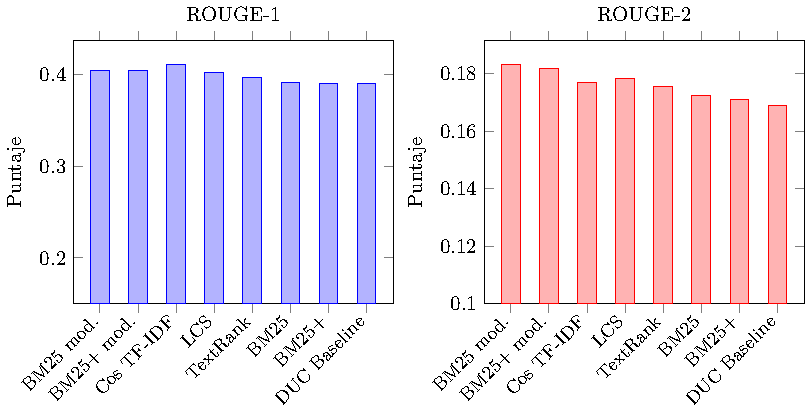
\includegraphics[width=1\textwidth]{rouge-scores.pdf}
    \caption{Comparación de métricas.}
\end{figure}


\section{Integración a Gensim}
La integración del módulo a Gensim\footnote{Pull request: \url{https://github.com/piskvorky/gensim/pull/324}
} se desarrolló a partir de su última versión, la 0.11.1-1. Se agregan a la biblioteca ambas funcionalidades descriptas anteriormente: la extracción de palabras claves y la generación automática de resúmenes extractivos.

En la integración se incluyen tres casos de uso:
\begin{itemize}
\item Generación de resúmenes automáticos dado un texto. En este caso la función requiere una cadena de texto con el documento a resumir, y devuelve el texto resumido. 
\item Selección de documentos más importantes dado un corpus. Este caso es similar al anterior, con la diferencia de que se recibe un listado de documentos (que pueden ser oraciones de un texto) y se devuelve un listado de aquéllos más importantes.
\item Obtención de palabras claves de un texto. En este caso se devuelve un listado de palabras clave dada una cadena de texto.
\end{itemize}


\section{Conclusiones}
En este trabajo se analizaron variantes al algoritmo de TextRank. A partir del mismo se propusieron e implementaron optimizaciones cuyos resultados fueron significativos: se obtuvo una mejoría del 2,92\% por sobre el método original. Este número es notable si se tiene en cuenta que TextRank por sí solo performa 2,84\% por sobre el estándar de comparación.

Las evaluaciones fueron hechas con las mismas técnicas y datasets utilizados en competencias internacionales, validando así las mediciones.

Queda para próximos trabajos explorar alternativas para la extracción de palabras claves, y el ensayo de distintos métodos algebraicos, haciendo uso del modelo del espacio vectorial.

Finalmente, la adaptación a la biblioteca de lenguaje natural Gensim también resultó sencilla gracias a las facilidades que provee su interfaz de programación y su gran cantidad de métodos.


\newpage
\section{Anexo I: modificaciones}
Además de las mejoras descriptas en la sección “Mejoras”, también se ensayaron otras ideas cuyos resultados no fueron tan destacables como los mencionados anteriormente.

Como se explicó anteriormente, las modificaciones apuntan a cambiar el criterio de similaridad entre oraciones. Algunas modificaciones que se tuvieron en cuenta son similares a la de subcadena común, que otorga puntajes de acuerdo a la cantidad de unidades léxicas en orden que estén presentes en las dos oraciones. Estas métricas son las usadas por el paquete Rouge, y los métodos de subsecuencia de palabras común, subsecuencia de palabras común con peso, bigramas comunes y SU4 son idénticos a los usados por los métodos ROUGE-L, ROUGE-W, ROUGE-2 y ROUGE-SU4.

Se diseñó un método que primero busca las palabras clave del documento para después asignarles un valor más alto en las ponderaciones; y un método que asigna puntaje adicional a aquéllas palabras que se mencionaron más recientemente.

Se implementaron también métricas de distancias de Levenshtein y una versión normalizada entre 0 y 1 teniendo en cuenta los extremos.

Finalmente, se experimentó también reemplazando el algoritmo de PageRank (que utiliza como solución el autovector asociado al valor asociado más grande de la matriz de similaridad) por el de HITS (que utiliza el vector singular asociado al valor singular más grande de la matriz); y también se probó aproximando la solución reduciendo el rango de la matriz.

\subsection{Resultados}
\begin{tabular}{ | l | l | l | l | l | l | l | }
\hline
	Método & ROUGE1 & ROUGE2 & ROUGESU4 & Mejora & Tiempo\\ \hline
	TextRank & 0.3983 & 0.1762 & 0.1948 & - & 0:00:25\\ \hline
	BM25 (Neg a epsilon) & 0.4042 & 0.1831 & 0.2018 & 2,92\% & 0:00:21\\ \hline
	BM25+ (Neg a epsilon) & 0.404 & 0.1818 & 0.2008 & 2,60\% & 0:00:21\\ \hline
	Cosine TF-IDF & 0.4108 & 0.177 & 0.1984 & 2,54\% & 0:03:30\\ \hline
	BM25+ (IDF = log(N/NI)) & 0.4022 & 0.1805 & 0.1997 & 2,05\% & 0:00:24\\ \hline
	BM25 (IDF = log(N/NI)) & 0.4012 & 0.1808 & 0.1998 & 1,97\% & 0:00:22\\ \hline
	Longest Common Substring & 0.402 & 0.1783 & 0.1971 & 1,40\% & 0:18:32\\ \hline
	LCW Subsequence & 0.4032 & 0.1773 & 0.1968 & 1,38\% & 0:01:02\\ \hline
	Weighted LCW Subsequence & 0.4032 & 0.1773 & 0.1968 & 1,38\% & 0:01:12\\ \hline
	BM25+ (Neg a cero) & 0.3992 & 0.1803 & 0.1976 & 1,36\% & 0:00:17\\ \hline
	BM25 (Neg a cero) & 0.3991 & 0.1778 & 0.1966 & 0,89\% & 0:00:22\\ \hline
	Distancia temporal & 0.3992 & 0.1762 & 0.195 & 0,48\% & 0:03:15\\ \hline
	Levenshtein & 0.3961 & 0.1781 & 0.1955 & 0,38\% & 0:27:49\\ \hline
	Longest Common Subsequence & 0.396 & 0.1775 & 0.1949 & 0,22\% & 0:28:08\\ \hline
	SU4 & 0.3955 & 0.1732 & 0.1924 & -0,73\% & 0:01:02\\ \hline
	Prioridad keywords & 0.3952 & 0.1721 & 0.1915 & -1,03\% & 0:07:13\\ \hline
	Peso de conceptos & 0.3953 & 0.1713 & 0.1914 & -1,14\% & 0:04:09\\ \hline
	Distancia temporal invertida & 0.3913 & 0.1725 & 0.1912 & -1,53\% & 0:03:05\\ \hline
	BM25 & 0.3916 & 0.1725 & 0.1906 & -1,57\% & 0:00:18\\ \hline
	HITS & 0.3914 & 0.1699 & 0.1898 & -2,03\% & 0:00:46\\ \hline
	BM25+ & 0.3903 & 0.1711 & 0.1894 & -2,07\% & 0:00:17\\ \hline
	HITS + DVS & 0.3912 & 0.1686 & 0.189 & -2,33\% & 0:00:46\\ \hline
	DUC Baseline & 0.39 & 0.1689 & 0.186 & -2,84\% & 0:00:01\\ \hline
	Bigramas comunes & 0.393 & 0.1633 & 0.1842 & -3,42\% & 0:00:50\\ \hline
	Weighted LCSubstring & 0.3755 & 0.1509 & 0.1729 & -8,79\% & 0:17:23\\ \hline
	Levenshtein normalizado & 0.348 & 0.1374 & 0.1565 & -16,28\% & 0:28:13\\ \hline
\end{tabular}




\bibliography{informe}{}
\bibliographystyle{babunsrt}


\end{document}
